%
% File acl2020.tex
%
%% Based on the style files for ACL 2020, which were
%% Based on the style files for ACL 2018, NAACL 2018/19, which were
%% Based on the style files for ACL-2015, with some improvements
%%  taken from the NAACL-2016 style
%% Based on the style files for ACL-2014, which were, in turn,
%% based on ACL-2013, ACL-2012, ACL-2011, ACL-2010, ACL-IJCNLP-2009,
%% EACL-2009, IJCNLP-2008...
%% Based on the style files for EACL 2006 by 
%%e.agirre@ehu.es or Sergi.Balari@uab.es
%% and that of ACL 08 by Joakim Nivre and Noah Smith

\documentclass[11pt,a4paper]{article}
\usepackage[hyperref]{acl2020}
\usepackage{times}
\usepackage{latexsym}
\usepackage{graphicx}
\renewcommand{\UrlFont}{\ttfamily\small}

% This is not strictly necessary, and may be commented out,
% but it will improve the layout of the manuscript,
% and will typically save some space.
\usepackage{microtype}

\aclfinalcopy % Uncomment this line for the final submission
%\def\aclpaperid{***} %  Enter the acl Paper ID here

%\setlength\titlebox{5cm}
% You can expand the titlebox if you need extra space
% to show all the authors. Please do not make the titlebox
% smaller than 5cm (the original size); we will check this
% in the camera-ready version and ask you to change it back.

\newcommand\BibTeX{B\textsc{ib}\TeX}

\title{The Dark Side of Language: Using NLP to Combat Hate Speech}

\author{ 
  Adam Hyman, 
  %\texttt{adamhyman@berkeley.edu} \\
  Shalini Chawla,
  %\texttt{schawla@berkeley.edu} \\
  Sreeram Ravinoothala \\
  %\texttt{sreeram@berkeley.edu} 
  }

\date{April 2023}

\begin{document}
\maketitle
\begin{abstract}
With the advent of social media, people have had access to propagate hate anonymously, making it more dangerous than ever as the impact is not contained by a social group or geographic area. It is very important for social media companies to accurately identify hateful content and remove it as the impact can be far fetched. In addition to just flag hateful content with a binary label, it is useful to identify the hate category, which can be further used to study any correlations between social-political events and its impact on specific categories of hateful content in online media. In this paper, we fine-tune three pre-trained large language models for a multi-label classification task to categorize user comments as toxic, severe\_toxic, obscene, threat, insult and identity\_hate. To help our models with accurately identifying the minority classes, we explore back translation as an option to augment existing data.

\end{abstract}

\section{Introduction}

In common language, “hate speech” refers to offensive discourse targeting a group or an individual based on inherent characteristics (such as race, religion or gender).

The adoption of Social media brings in different views of many people. One of the primary issues bleeding the social media community is hate speech. Hate speech brings lot of negativity in people that if not curtailed can spiral into bigger issues like what we see around us in many cases. Hate speech can be targeted against individual, community, ideology etc. The social platforms with so many resources at hand are able to take care of it though much more is needed to cut it at the root.

With the advances in AI/ML, many of the social media platforms have done a lot of great work in controlling the proliferation of hate speech by making use of classification algorithms but there is much more to be done to reduce the exposure to a great extent.

Hate speech on social media platform is well known and the platforms are employing different techniques to bring the exposure down. They are successful in many ways but classifying the content to check if it indeed is hate is very complex as it depends on the context as well as whether its used loosely. There is lot of research done or going on classifying the text as well as augmenting such text.

The ability in building accurate models to correctly classify hateful content is a challenging task due to the limited availability of labeled data required for training. The training data needs to be labeled by human annotators. In addition to being a tedious task, it also exposes the annotators to the disturbing content in the data they are required to label. The public data sets available today are highly imbalanced and have very limited samples for some of the minority categories including threat, obscene and severe\_toxic compared to the large amount of non-toxic samples. We follow two approaches to deal with the limitations of data availability.

1) We use pre-trained large language models and fine tune them for a classification tasks. Using a pre-trained model gives us the ability to use smaller amount of training data to achieve the same performance that would have required a much larger training data set with a classifier built from ground up.

2) We use data augmentation to further balance our data set across the toxic classification categories. We have three minority categories: threat, severe-toxic and identity\_hate that have very low representation in our training data set. We use the TOXIGEN data set to augment data for the identity\_hate class. To augment data for the other classes, we use reverse translation to generate additional samples from the existing data. 



\section{Background}
The task of toxic content classification has been tackled before using many different approaches. The availability of quality labeled data has been widely accepted as a limitation in the ability to create accurate models for toxic content classification.
(Rastogi et al.) has explored generating synthetic data using EDA and back translation to augment the training data and reported improved recall and F1 scores. (Hartvigsen et al., ACL 2022) have used GPT-2 to generate synthetic identity\_hate data to help improve the claasification accuracy of implicit conent. 


\section{Data}

\subsection{Source Data Set}
We use the jigaw dataset from kaggle competition that was derived out of reddit data. The data set consist of 3 files that includes the labeled training data, test data and the test labels. We combine the test data and labels file by joining them on the unique comment identifiers. The training data set has 159,000 samples while the test data set has 60,000 samples. We convert the comments into lowercase and clean the contents by removing punctuation and special characters. Once processed both are training and test data file  consist of the text comments and binary labels for the 6 categories listed below.

\begin{itemize}
\item toxic
\item severe\_toxic
\item obscene
\item threat
\item insult
\item identity\_hate
\end{itemize}

\subsection{Data Balancing}
Our source data is highly imbalanced. Out of the 6 labeled classes, 3 are majority classes with and 3 are minority classes.
\begin{table}
\centering
\begin{tabular}{l r}
\hline
\textbf{Label} & \textbf{Count}\\
\hline
\verb|toxic| & 159000 \\
\verb|severe_toxic| & 1500 \\
\verb|obscene| & 500 \\ 
\verb|threat| & 500 \\ 
\verb|insult| & 500 \\
\verb|identity_hate| & 500 \\
\hline 
\end{tabular}
\caption{Distribution of toxicity labels in the source data set.}
\end{table}

\begin{figure}[h!]
\centering
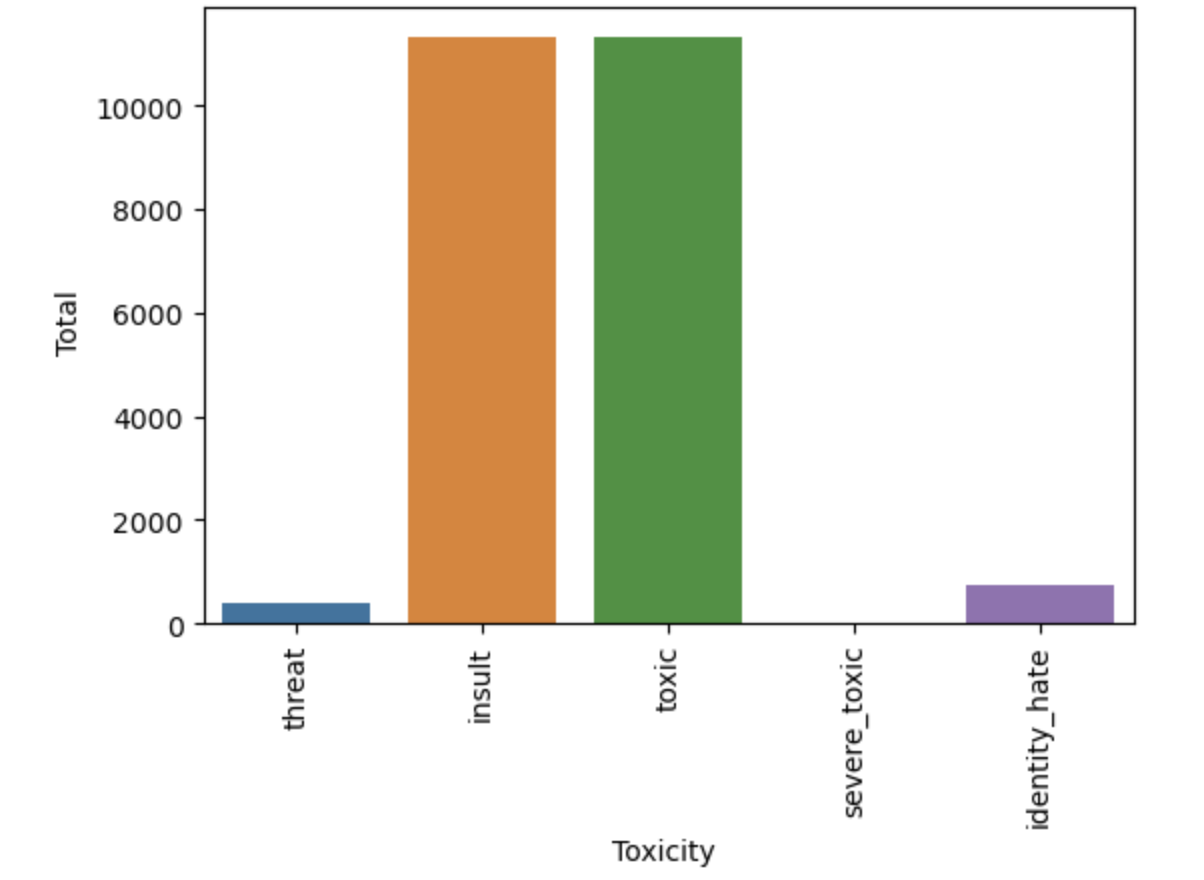
\includegraphics[width=50mm,scale=0.5]{label_counts.png}
\caption{Toxicity Label Count}
\label{Fig1. label count vs toxicity}
\end{figure}

\subsection{Undersampling Majority Class Data}
To balance the data set for the 6 classes being identified, we use a combination of strategies. We undersample two of two majority classes severe\_toxic and obscene to select 2000 random samples each from the original training data set. Since the label toxic is set to True if any of the 

\subsection{Augmenting Minority Class Data}
To bring the available training data for minority classes to be closer in count to the majority classes more balanced To augment the data for minority classes identity\_hate, we chose to augment with the data available from the TOXIGEN dataset[2]


\section{Methods}

\subsection{Baseline Model}
Our baseline model is BERT base model(cased). We fine-tune the model on the full training data set that has been split into training and validation using 80:20 split and stratified on the 6 label classes. We add a hidden layer with 200 neurons and dropout layer with 0.3 before our final classification layer with 6 outputs to perform a multi label classification. We train the model for 2 epochs using learning rate of .00005 and batch size of 32.

As expected, the model performs really poorly for our 3 minority classes.

\begin{table}
\centering
\begin{tabular}{lrrr}
\hline
\textbf{class} & \textbf{prec} & \textbf{recall} & \textbf{f1-score}\\
\hline
\verb|toxic| & 0.62 & 0.40 & 0.49 \\
\verb|severe_toxic| & \textcolor{red}{0.00} & \textcolor{red}{0.00} & \textcolor{red}{0.00} \\
\verb|obscene| & 0.66 & 0.32 & 0.43 \\
\verb|threat| & \textcolor{red}{0.00} & \textcolor{red}{0.00} & \textcolor{red}{0.00} \\
\verb|insult| & 0.65 & 0.25 & 0.36 \\
\verb|identity_hate| & \textcolor{red}{0.00} & \textcolor{red}{0.00} & \textcolor{red}{0.00} \\
\vspace{2\baselineskip}\\
\verb|micro avg| & 0.64 & 0.31 & 0.42 \\
\verb|macro avg| & 0.32 & 0.16 & 0.21 \\
\verb|weighted avf| & 0.58 & 0.31 & 0.40 \\
\verb|samples avg| & 0.04 & 0.03 & 0.03 \\
\hline
\end{tabular}
\caption{Baseline Model - Classification Report}
\end{table}


\subsection{T5}
Another model we used is T5-small. We used the model on fine tuned baseline training dataset similart to BERT which was stratified. We used huggingface Transformers library to achieve this task. The pretrained T5 model is used to do text-text conversion. As part of the multilabel classification a language modeling head is used on top of the decoder. The model was run 2 epochs with 8 and 16 batch size. Both the runs gave almost similar results. Table 3 provides the f1 scores, precision and recall across all 6 label classes. 

It can be noted that certain classes like insult and identity hate have 0 f1-score whereas the hamming loss seems to be better. The two classes whose f1 scores are 0 depicts that this model is not good for this job. This can be due to the imbalance in the data for those two classes.


The metrics that are captured as part of training and validation are as below. The validation f1 score shows that the model is producing a very good prediction.

2 epochs, 8 batch \\
epoch 1:
\begin{itemize}
\item Training loss: 0.1471774057341023
\item Val loss: 0.08538059349774901
\item Val accuracy: 0.9676944287773391
\item Val micro f1 score: 0.6594594594594594
\item \-\-\- Best Model. Val loss: -inf - 0.6594594594594594
\end{itemize}
echo 2:
\begin{itemize}
\item Training loss: 0.08286546394057061
\item Val loss: 0.08029992060314782
\item Val accuracy: 0.9676317603559567
\item Val micro f1 score: 0.6922290388548057
\item \-\-\- Best Model. Val loss: 0.6594594594594594 -0.6922290388548057
\end{itemize}

Hamming loss: 0.04526198962045895


\subsection{XLNet}

\section{Results and Discussion}
Metrics were captured across multiple models that were tested as shown in Table ~\ref{table:results}. Each model was run for multiple epochs to ensure proper outcome of metrics. Bert model was fine tuned by unfreezing different number of layers inorder for BERT to learn the toxic data. The data clearly shows how the model has improved with respect to F1 score as well as AUC-ROC numbersi and hamming loss. 

T5 was applied on unbalanced data and balanced data. But, the metrics are not too significantly different to say one of them is better.

Similarly XLNet model was applied on both unbalanced as well as balanced dataset.

There is a clear indication of how each model shines given a balanced dataset. XLNet clearly shows its predictions are way better than the other two models.

\begin{table} {p{0.35\linewidth} | p{0.6\linewidth} | p{0.6\linewidth} | p{0.6\linewidth} | p{0.6\linewidth} | p{0.6\linewidth} | p{0.6\linewidth} | p{0.6\linewidth} | p{0.6\linewidth} | p{0.6\linewidth}}
\centering
\begin{tabular}{lrrr}
\hline
\textbf{Model} & \textbf{Macro F1-Score} & \textbf{Macro AUC-ROC} & \textbf{Toxic AUC-ROC}  & \textbf{Super Toxic AUC-ROC} & \textbf{Obscene AUC-ROC} & \textbf{Threat AUC-ROC} & \textbf{Insult AUC-ROC} & \textbf{ID Hate AUC-ROC} & \textbf{Hamming loss}\\
\hline
\verb|Bert Base| & 0.2 & 0.56 & 0.66 & 0.5 & 0.63 & 0.5 & 0.61 & 0.5 & 0.03 \\
\verb|Bert Bal| & 0.05 & 0.51 & 0.57 & 0.5 & 0.5 & 0.49 & 0.5 & 0.5 & 0.03 \\
\verb|Bert 2 layers Base| & 0.5 & 0.74 & 0.88 & 0.6 & 0.87 & 0.57 & 0.8 & 0.02 \\
\verb|Bert 2 layers Bal| & 0.42 & 0.86 & 0.85 & 0.79 & 0.87 & 0.91 & 0.83 & 0.89 & 0.05 \\
\verb|Bert 4 layers Base| & 0.55 & 0.78 & 0.9 & 0.59 & 0.86 & 0.71 & 0.88 & 0.72 & 0.03 \\
\verb|Bert 4 layers Bal| & 0.44 & 0.87 & 0.6 & 0.88 & 0.87 & 0.92 & 0.83 & 0.88 & 0.05 \\
\verb|Bert 6 layers Base| & & & & & & & & & \\
\verb|Bert 6 layers Bal| & 0.5 & 0.83 & 0.87 & 0.73 & 0.83 & 0.88 & 0.79 & 0.9 & 0.03 \\
\verb|Bert All layers Base| & 0.49 & 0.77 & 0.9 & 0.73 & 0.89 & 0.49 & 0.88 & 0.73 & 0.03 \\
\verb|Bert All layers Bal| & 0.51 & 0.89 & 0.89 & 0.87 & 0.88 & 0.9 & 0.87 & 0.91 & 0.04 \\
\verb|T5 Base| & 0.07 & 0.59 & 0.53 & 0.94 & 0.51 & 0.58 & 0.5 & 0.5 & 0.04 \\
\verb|T5  Bal| & 0.12 & 0.61 & 0.77 & 0.92 & 0.52 & 0.49 & 0.5 & 0.5 & 0.05 \\
\verb|XLNet Base| & & & & & & & & & \\
\verb|XLNet  Bal| & 0.42 & 0.89 & 0.89 & 0.83 & 0.89 & 0.95 & 0.88 & 0.92 & \\
\vspace{2\baselineskip}\\
\hline
\end{tabular}
\caption{T5  Model - Classification Report}
\label{table:results}
\end{table}
\section{Error Analysis}

\section{Conclusion}

\section*{References}
Rastogi, Chetanya, et al. “Can We Achieve More with Less? Exploring Data Augmentation for Toxic Comment Classification.” ArXiv:2007.00875 [Cs], 2 July 2020, arxiv.org/abs/2007.00875. Accessed 31 Mar. 2023.\\\\
Thomas Hartvigsen, Saadia Gabriel, Hamid Palangi, Maarten Sap, Dipankar Ray, and Ece Kamar. 2022. ToxiGen: A Large-Scale Machine-Generated Dataset for Adversarial and Implicit Hate Speech Detection. In Proceedings of the 60th Annual Meeting of the Association for Computational Linguistics (Volume 1: Long Papers), pages 3309–3326, Dublin, Ireland. Association for Computational Linguistics.

\end{document}
